% Le titre de la partie
\section[Validation]{Tentatives de prédiction des cambriolages dans la ville de Chicago et commentaires}

%%%%%%%%%%%%%%%%%%%%%%%%%%%%%%%%%%%%%%%%%%%%%%%%
% Première diapo (avec des équations)
%%%%%%%%%%%%%%%%%%%%%%%%%%%%%%%%%%%%%%%%%%%%%%%%
\begin{frame}
    \frametitle{Validation du modèle}
    \framesubtitle{}
    \begin{block}{Résultats}
         \begin{itemize}
            \item Correspondance avec les données réelles
            \item Qualité du modèle (erreur relative faible de 2.44\%)
            \item Pertinence du processus de Hawkes
            \item Utilité pour la prévision ?
            \end{itemize}
  
  \end{block}    
\end{frame}

\begin{frame}
    \frametitle{Utilisation du modèle}
    \framesubtitle{Prévisions du nombre de cambriolages en 2021}
    \begin{block}{Résultats}
         \begin{itemize}
            \item Nombre réel: 107 
            \item Nombre prédit: 109
            \end{itemize}
  \end{block}    
\end{frame}

\begin{frame}
    \frametitle{Application du modèle}
    \framesubtitle{}
        \begin{figure}
            \centering
            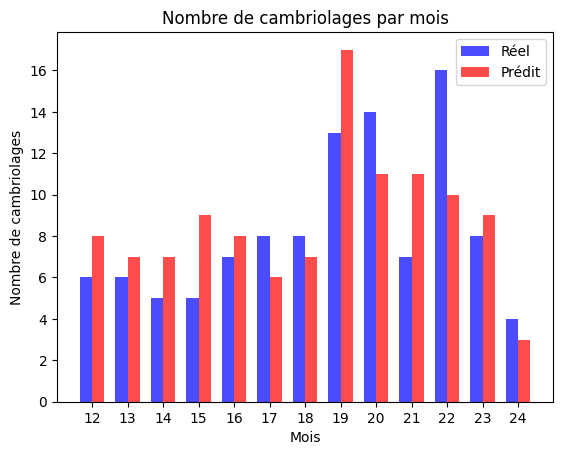
\includegraphics[width=0.6\linewidth]{figures/téléchargement (4).png}
        \end{figure}
\end{frame}

\begin{frame}
    \frametitle{Utilisation du modèle}
    \framesubtitle{Limites du modèle}
    \begin{block}{Limites du modèle}
        \begin{itemize}
            \item Simplification du processus réel
            \item Hypothèses du modèle
            \item Prédictions à long terme
            \item Sensibilité aux paramètres
            \item Difficulté de calibrage
            \item Manque d'explications causales 
        \end{itemize}
    \end{block}    
\end{frame}


\begin{frame}
    \frametitle{Utilisation du modèle}
    \framesubtitle{Limites du modèle}
    \begin{alertblock}{Peut-on envisager l'utilisation d'un tel modèle dans la vie courante? L'exemple de PredPol}
        \begin{figure}
            \centering
            
\includegraphics[width=0.6\linewidth]{figures/CorteX_predpol_slogan.jpg}
            \caption{www.predpol.com}
        \end{figure}
    \end{alertblock}
\end{frame}

\begin{frame}
    \frametitle{Utilisation du modèle}
    \framesubtitle{Limites du modèle}
    \begin{alertblock}{Peut-on envisager l'utilisation d'un tel modèle dans la vie courante? L'exemple de PredPol}
        \begin{figure}
            \centering
            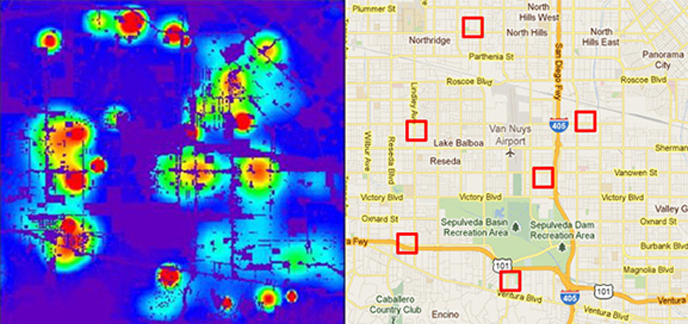
\includegraphics[width=0.6\linewidth]{figures/i_predpol.jpg}
            \caption{www.predpol.com}
        \end{figure}
    \end{alertblock}
\end{frame}

\begin{frame}
    \frametitle{Fin du TIPE}
    \framesubtitle{}
        \centering
        \Large{Merci pour votre attention!}
\end{frame}



